\documentclass[10pt,a4paper]{article}
\usepackage{graphicx}
	\graphicspath {
		{./images/}
	}

\usepackage{hyperref}
\hypersetup{
    colorlinks=true,
    linkcolor=blue,
    filecolor=magenta,      
    urlcolor=cyan,
}

\author{Jimmy Tang}
\date{2017-2018 Summer Research}
\title{USB Protocol Packet Sniffing}

\begin{document}

\maketitle
\pagenumbering{gobble}
\tableofcontents

\newpage
\pagenumbering{arabic}
\section{Summary}
This document is intended to be used as a reference that will detail the important parts of this research project and not written to be read in a specific order. The target audience is an Undergraduate Computer Science or Software Engineering student with little to no experience in hardware design. Continue with Programming and Flashing the FPGA 
\section{Equipment}
\subsection{Equipment Checklist}
\begin{enumerate}
	\item FPGA (Xilinx Spartan 6 XC6SLX16 CSG324C)
	\item Development Board (Nexys3 Development Board)
	\item USB Interface
	\item Beagle USB 5000 Super Speed
\end{enumerate}
\subsection{Technology Short Description}
\subsubsection{Verilog}
Verilog is a Hardware Description Language (HDL) used predominately in this research project as a means to describe the hardware implementation of the USB 1.1 Function core and the interface between the development board to USB interface to the host computer. Verilog files are generally suffixed by .v and closely resembles the programming language C. Remember that everything done in hardware is done in parallel so work with \emph{finite state machine} as opposed to for loops and flow statements (flow and iteration works differently in Verilog)
\subsubsection{FPGA}
The FPGA is a special chip that takes a bit stream generated via a HDL file and configures itself to act as that particular hardware implementation. FPGAs are reconfigureable as opposed to Application Specific Integrated Circuit (ASIC) which is desirable in research projects, and prototyping where a lot of testing occurs. Every FPGA has some number of in and out pins which forms the connection to the outside world. These pins need to be constraint via a constraint file, there exists a template Nexys3 Development Board constraints file (suffixed with .ucf) that can be found in the documentation for the Nexys 3 Development Board.
\subsubsection{Xilinx ISE}
Xilinx ISE is a free IDE offered by Xilinx which will allow you as the developer to Synthesise, Implement, Generate a programming file, and flash the FPGA from this program. Xilinx ISE comes with an inbuilt text editor with syntax highlighting and templates for adding in HDL source files.
\subsubsection{Beagle USB 5000 Super Speed}
This is a specialty device used to examine the USB 2.0 and 3.0 protocol between host and device to observe packets passing through. Fairly simple to be used, will be discussed in depth in a later section.
\section{Getting Started}
\subsection{Setting up the project}
Download and run the \href{https://www.xilinx.com/support/download/index.html/content/xilinx/en/downloadNav/design-tools/v2012_4---14_7.html}{Xilinx ISE Design program}, download the free license or use the one provided in the git repository. Create a new project at any location and under "Evaluation Development Board" choose the option "Spartan-6 SP601 Evaluation Platform". If you cannot find it, see figure \ref{fig:Evaluation Platform} for a screen capture.

\begin{figure}
	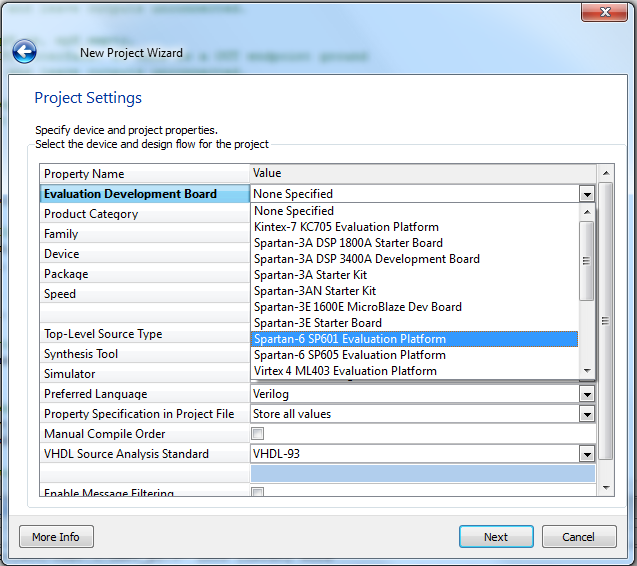
\includegraphics[width=12cm,height=10cm]{Evaluation_Platform.PNG}
	\caption{Evaluation Platform}
	\label{fig:Evaluation Platform}
\end{figure}
\subsection{Programming and Flashing the FPGA}
\subsubsection{Xilinx ISE}
Programming the Nexys 3 Development Board using Xilinx ISE \\ \\
see figure ~\ref{fig:configure_target} which can be found after opening up the ISE program and loading up a project with the Verilog files you want to program into the board. By default, this window should be found in the middle left of the window.\\ \\
\begin{figure}[h!]
	%~\ref{fig:configure_target}
	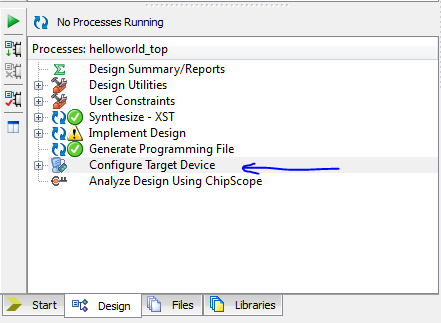
\includegraphics[width=12cm,height=10cm]{configure_device.PNG}
	\caption{Synthesizing the design, placing and routing, and opening up iMPACT}
	\label{fig:configure_target}
\end{figure}

Below is a list of instructions on how to use iMPACT to program the Nexys 3 Development Board.
\begin{itemize}
	\item iMPACT opens up
	\item perform boundary scan
	\item initialise the JTAG chain
	\item programming file (.bit extension)
	\item Do not Flash PROM
	\item apply to device 1
	\item right click on Xilinx chip and select program
\end{itemize}

If you had used the helloworld\_top.v file, you should be able to press the BTND at location C9 to turn on the LD1 at location T9 LED, and flick the switch SW0 at location T10 to turn on the LD0 at U16 LED

\subsubsection{Adept}
Programming the Nexys3 Development Board could also be done using Adept provided by Digilent. See the tutorial found under 'Reference Materials' for further information.\\ \\
The process is incredibly simple, install the program onto your desktop, connect the Nexys 3 board via the USB cable provided, run the program, choose the bit file, and then press the 'program' button. \\
If the device cannot be found, ensure the Nexys 3 board's power switch is on and click on the 'Initialize Chain' button 

\subsection{Examining USB protocol packets using the Beagle USB 5000}
\subsubsection{Requirements}
\begin{itemize}
	\item USB Drivers: TotalPhaseUSB-v2.15
	\item Packet Analyser Software: Data Center 
	\item Firmware Updates: Beagle Update Utility (Optional)
\end{itemize}
\subsubsection{Beagle 5000 Setup}
\href{https://www.totalphase.com/support/articles/200801823-Getting-Started-Beagle-USB-5000-v2-SuperSpeed-Standard-Protocol-Analyzer}{Guide to Getting started with the Beagle USB 5000.}
Download the USB Drivers for your machine, and the Data Center software. Optionally the \href{https://www.totalphase.com/products/beagle-5000-firmware-utility/}{firmware update} could be downloaded and installed from here. \\
Connect all cables to match figure \ref{fig:Beagle USB 5000}. \\
The USB port type B labeled as 'ANALYSIS' should be connected to a USB hub that is connected to the Computer that has the USB Drivers and Data Center software installed.\\
The USB port type B which supports USB 3.0 labeled as 'HOST' acts as the end of the device to be analysed. The USB type A port labeled 'DEVICE' simply hosts the device to be analysed. In the context of this document, this would be the developed USB device implemented on the Nexys3 Development Board. \\
The 12V/2A powers the Signal Analyser and is to be connected to a mains power point.
\begin{figure}[h]
	\includegraphics[width=12cm, height=10cm]{beagle_5000.jpg}
	\caption{Beagle USB 5000 Setup}
	\label{fig:Beagle USB 5000}
\end{figure}

\subsubsection{Capturing Packets}
Having installed the USB Drivers and software and properly connected up the Beagle 5000, capturing USB packets is easy. Below is a set of steps to take, refer to figure \ref{fig:Data Center Setup} to find out where the relevant configuration buttons are. Take extra notice of the arrows drawn, pressing the B button will open up the setup window set the capture mode to USB 2.0 Only, and to trigger immediately (pressing D the play button will also begin capturing packets straight away).

\begin{enumerate}
	\item Run the Data Center program
	\item Setup to examine USB 2.0 and to trigger immediately (B)
	\item Default Capture settings should be okay (C)
	\item Scan and connect the Beagle 5000 (A)
	\item Click run (D)
	\item Insert the target USB device (example Pen drive or keyboard/mouse)
	\item Pause when desired packets are observed
	\item (optional) export data to another format such as csv (hotkey: Ctrl+E)
\end{enumerate}

\begin{figure}[h]
	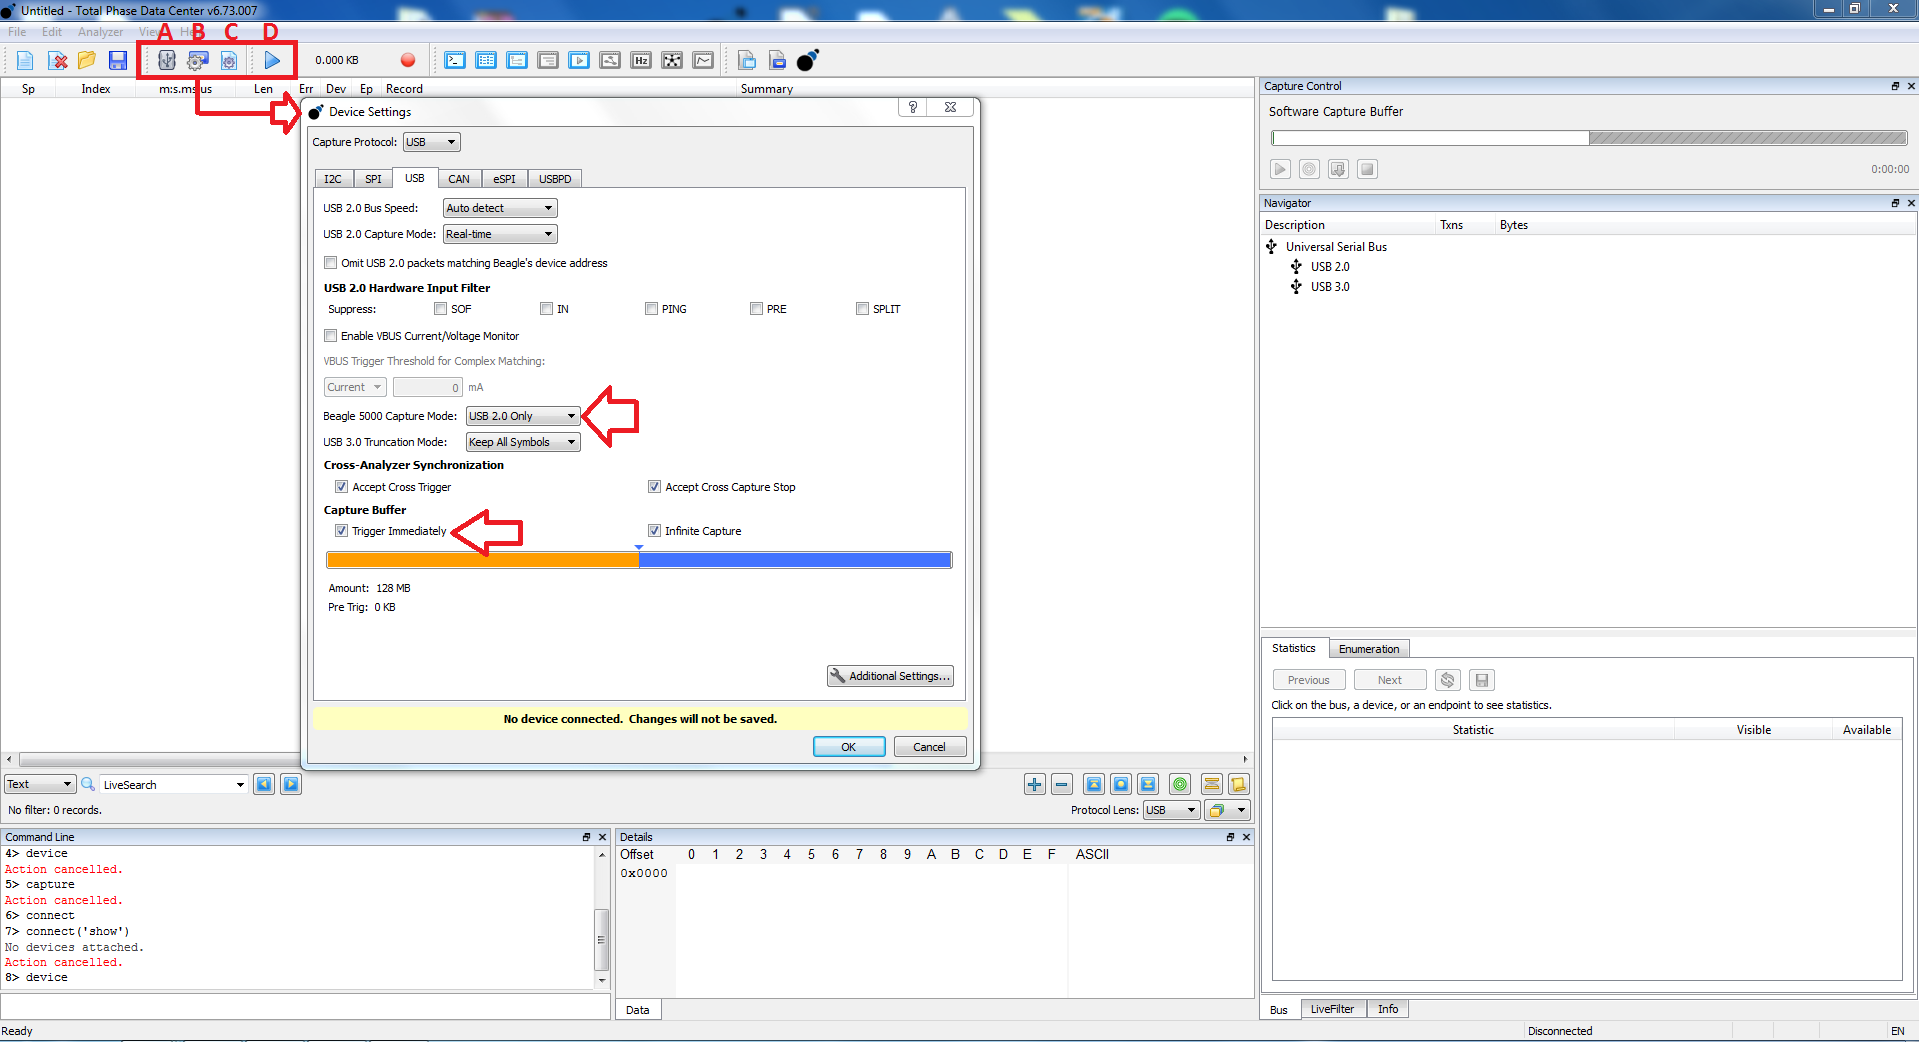
\includegraphics[width=12cm,height=10cm]{Data_Center.PNG}
	\caption{Data Center Setup}
	\label{fig:Data Center Setup}
\end{figure}

Once captured packets, the window should resemble figure \ref{fig:Retrieved Packets and Applying Filters} where 'A' is a window full of packets pertaining to USB protocol and 'B' is a window for applying filters. It is recommended that filters are used in order to have better insight into the packets to be observed.

\begin{figure}[h]
	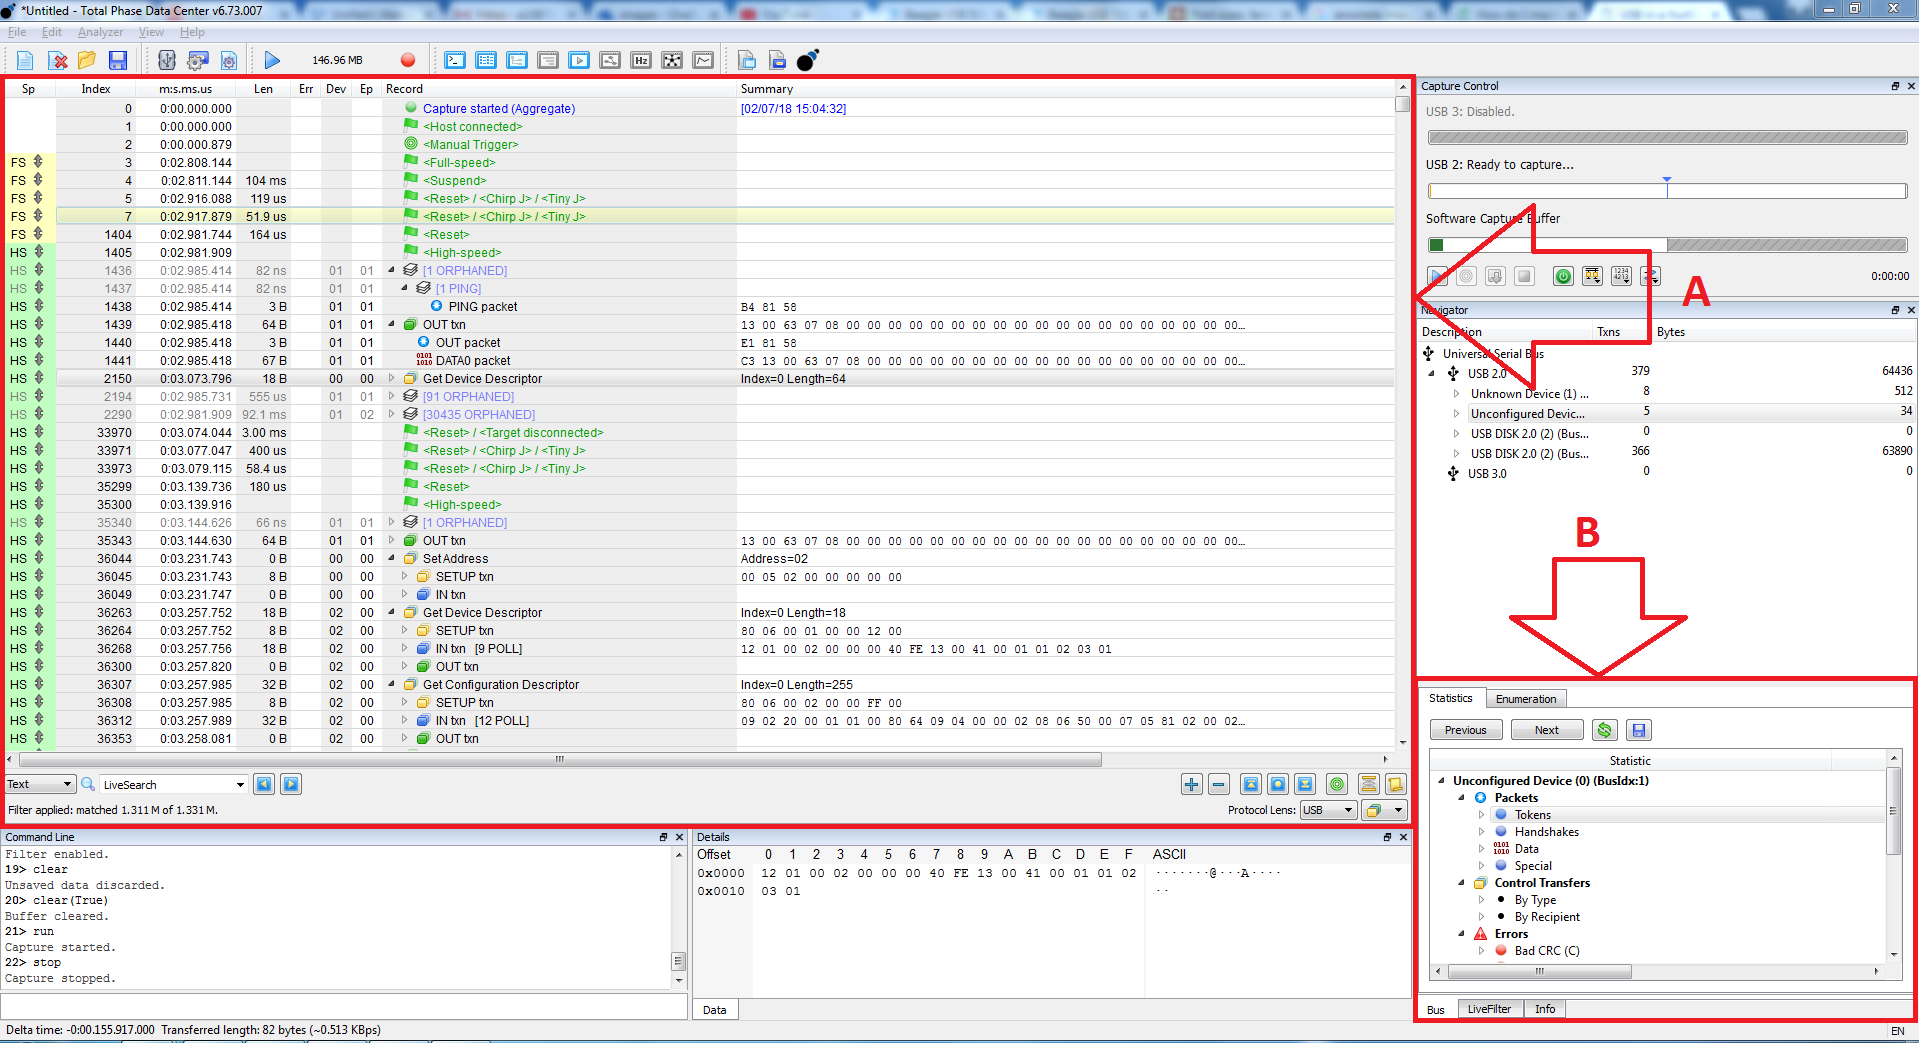
\includegraphics[width=12cm,height=10cm]{Data_Center_Packets.PNG}
	\caption{Retrieved Packets and Applying Filters}
	\label{fig:Retrieved Packets and Applying Filters}
\end{figure}

\subsection{Example Hardware Implementations}
\subsubsection{Hello World in Hardware}
Simple programming of the Nexys3 Development board to turn on LEDs via pressing down buttons and toggling switches. This section will go through importing Verilog files into Xilinx ISE, constraining a design with a .ucf file, simulating a design with a test bench, and some basic Verilog code.
\subsubsection{Linear Feedback Shift Register (LFSR)}
The Linear Feedback Shift Register (LFSR) is a hardware implementation of a pseudo-random number generator. Good practice for getting used to writing a HDL file for flashing a development board hosting an FPGA. The LFSR requires a seed (starting point) and a feedback polynomial (find this online). My implementation has a hard coded seed of 10101010b for testing purposes. Note that this implementation will not work with a starting value of 00000000b because every next value depends on the previous value, if all values are zeros then the next set of values will also be zero resulting in a cycle.
\subsubsection{Clock/Frequency Divider}
The Clock/Frequency Divider is a way to slow down the native speed of the clock internal to the Nexys3 Board. This core will be useful for examining the output of the LFSR by causing the device to count slower allowing for humans eyes to examine the changing of state. Clock division is done by updating the next clock's output anytime the current clock's output is driven high. Given that the Nexys3 board runs on a 100MHz clock, if we were to slow it down to a reasonable length of time and output the value of the LFSR to the LEDs onboard the development board, the changing states will be visible. Dividing the clock by 27 times will give us a period of roughly 1.3 seconds.
$$ clock speed = 100MHz = 100,000,000 \frac{cycles}{second} $$
$$ \frac{clock speed}{2^{27}} \approx 0.745 \frac{cycles}{second} $$
$$ period = 1.342 \frac{seconds}{cycle} $$
\subsubsection{Bi-Directional Data Lines} 
All USB devices have bi-directional data lines, in the case of USB 1.1 and 2.0, there are two data lines d+ and d- which are used to transmit and receive serial data. The USB 1.1 core provided by opencores.org will handle the sending and transmitting of data packets however the connection between the development board and USB interface must be written and interfaced between the USB 1.1 function core and the Nexys3 board. This is done via the use of Bi-Directional data lines of which a simple Verilog file will demonstrate this property. \\ \\
The basic concept is to have a register constantly loading in the the value coming from the data line and a transmission wire that is either connected or disconnected depending on an internal write enable pin. The transmission wire is implemented using a multiplexer with two inputs: data to be sent out; high impedance (Z). High impedance being the same as a disconnected wire.
\subsubsection{Finite State Machine} 
Finite State Machines are the Flow statements of hardware.
\subsubsection{Module Instantiations} 
Module Instantiation is the basic idea that is required to create the top module that interfaces between the USB 1.1 Function Core and the Nexys3 Development Board and is important to any Hardware Development. Analogous to object instantiation in an object orient programming language such as C++ or Java
\section{Research Findings}
\subsection{USB Protocol and Enumeration}
USB devices must go through an enumeration process which will allocate a device ID in the range from [1:128] with ID=0 being reserved for newly connected devices. The USB protocol works by using endpoints and descriptors to describe the functionality of a particular USB device, notably HID devices such as keyboards, and mice loop between endpoints 1 and 2 when transferring polled data.\\

I suspect that the enumeration process will be dealt with by the USB 1.1 function core however information regarding the device, configuration, and endpoint descriptors are missing or have yet to be filled out. There is a reasonable chance that somewhere in the USB 1.1 function core is a piece of ROM that is used to fetch the descriptors from but the question regarding where that ROM lies in the USB core eludes me.\\

So far, I have connected up the Nexys 3 Development Board hosting the USB 1.1 function core, bi-directional lines, and LEDs (programmed state, and logic of the data lines D+ and D-) to receive a setup transaction. There are no acknowledgments to be found in response to the setup packets which is to be expected as I have not described how the USB 1.1 function core will behave (what to reply).\\

Note that VBus and GND pins coming from the USB interface need not be connected, logic lines D+ and D- will still work without connecting these two wires. A common GND pin may still need to be considered when using separate computers for Analysis and Experiment. Possible reason packets were still sent may be because Analysis and Experiment computers were the same. \\

\subsection{what to do next}
Date written: 16/02/2018
\begin{enumerate}
	\item work with the iCE stick, see if all Verilog project files could be transferred onto that development board.
	\item Order in a USB 1.1 PHY transceiver from \href{https://au.mouser.com/Semiconductors/Interface-ICs/USB-Interface-IC/_/N-45lw3Z1yzvvqx?P=1yxy7lq&pop=3nh2d&Ns=Pricing|0}{au.Mouser.com} or another retailer.
	\item Instantiate a USB 1.1 PHY following \href{http://www.xess.com/projects/fpga-usb-v2-project/}{this guide}
\end{enumerate}

\subsection{Experiment Setup}
\underline{Connection Setup, make sure to reference figure \ref{fig:Experiment Setup}. }\\
\textbf{Experiment Computer:} the computer of which the USB device is connected to. \\
\textbf{Analysis Computer:} The computer that will flash the FPGA, and run Data Center \\
\textbf{Note} that the Experiment Computer and Analysis Computer could be the same computer, there should be no problems having this setup this way.
\begin{enumerate}
	\item 'A' : Connect mini USB port to the Experiment Computer. Connect this port and flash the device
	\item 'B' : Two LEDs will show the state of the data lines D+ and D- at 'D1' on the photo. It is expected that D- (LED[6]) is at 3.3V and D+ (LED[7]) is at 0.0V as these are the conditions for a Full Speed connection. \href{http://www.beyondlogic.org/usbnutshell/usb2.shtml}{more information regarding speed identification can be found here.}
	\item 'C' : These 4 LEDs (LED[3:0]) have been programmed to indicate whether the device was successfully flashed or not. All 4 LEDs should be in the on state.
	\item 'D1' : This is where the Beagle 5000 will connect to the Nexys 3 Development Board. JD1 = D-; JD2 = D+; Make sure to not connect the red (VBus 5.0V) and black (GND 0.0V) wires as there is potential to damage any of the components.
	\item 'D2' : The USB interface soldered onto a prototyping board, the Yellow wire = D+; Green wire = D-;
	\item 'E' : Acts as the other end to the device, connect this to the Experiment Computer
	\item 'F' : Analysis data leaves through this port, connect the other end to the Analysis Computer
	\item 'G' : Power, connect this end to a power board.
\end{enumerate}

\begin{figure}
	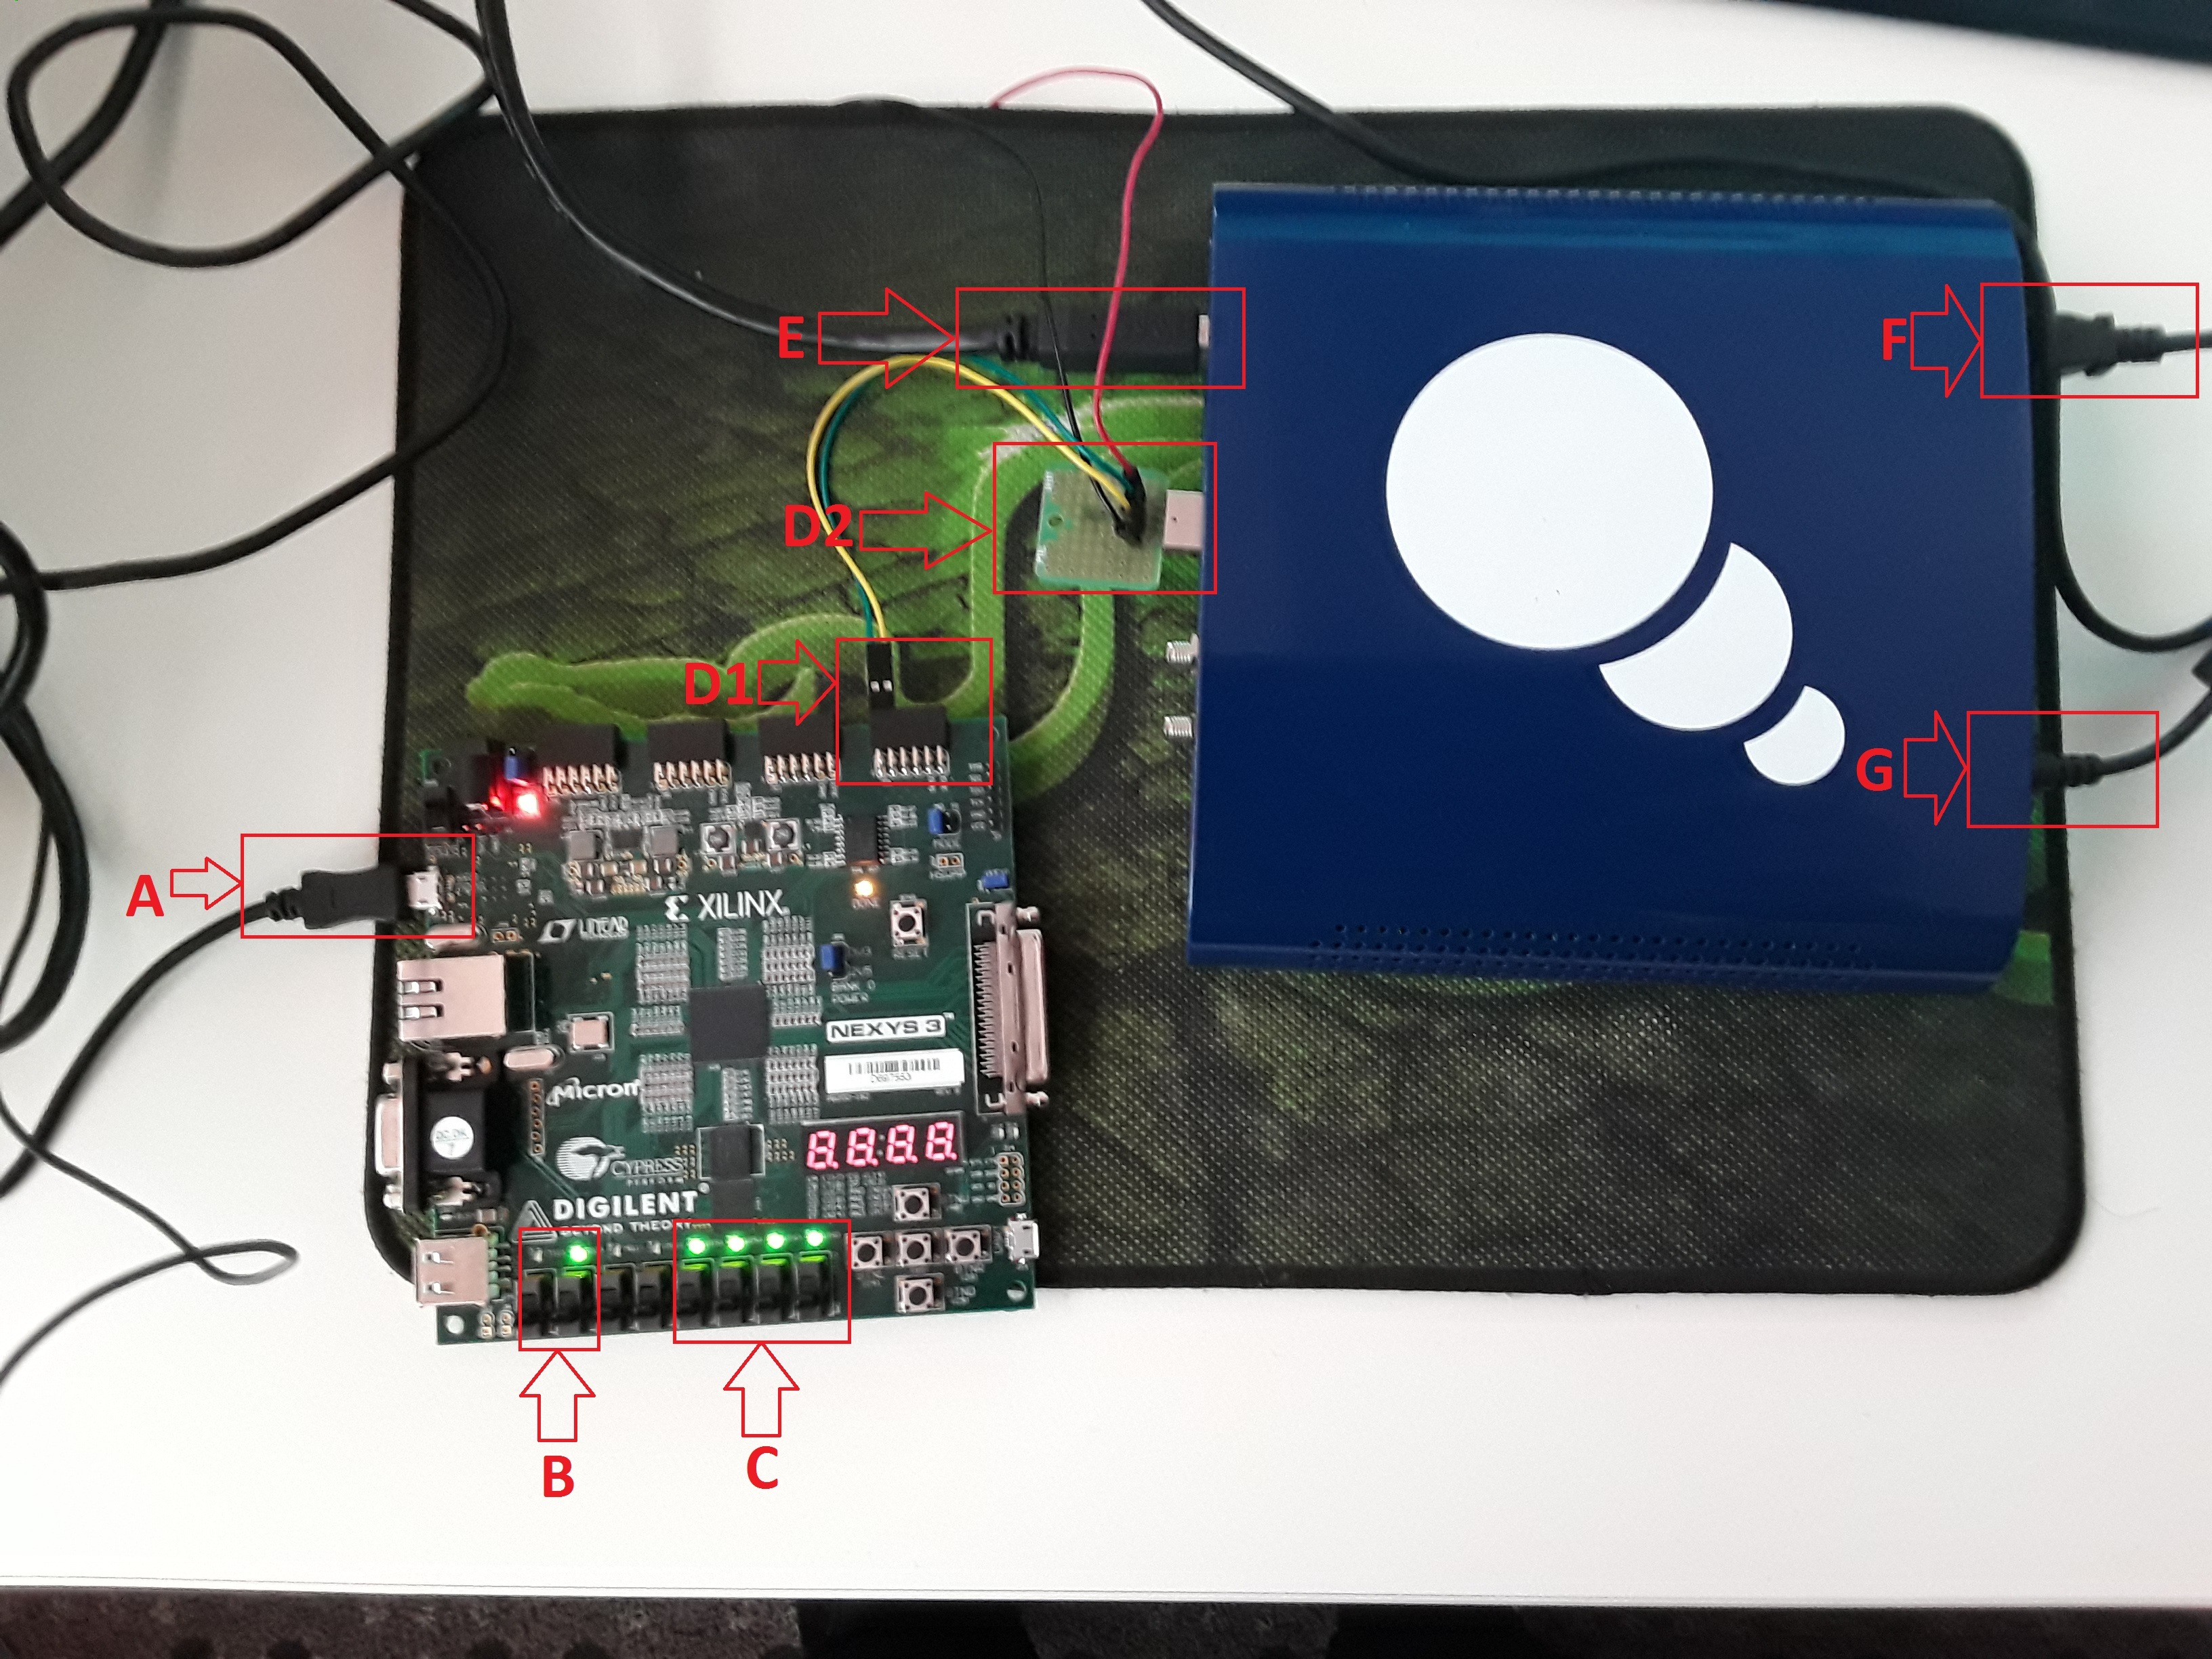
\includegraphics[width=12cm,height=10cm]{Experiment_Setup.jpg}
	\caption{Experiment Setup}
	\label{fig:Experiment Setup}
\end{figure}

\subsection{Current Situation}
\underline{The current situation as of the week starting 12/Feb/2018}\\\\
The Nexys 3 Development board has been flashed with the latest version of the HDL file and connected up to a host computer. The result turns out to be that Windows 7 would recognise that a device has been detected but malfunctioned. This leads me to attaching the Beagle 5000 inbetween and examining the packets passing through host to device. There appears to be no ACK packet (see figure \ref{fig:Lack of ACK packets}) being received upon experimenting with the current hardware setup. A post to the \href{https://electronics.stackexchange.com/questions/355777/lack-of-ack-packets-appears-to-cause-custom-usb-core-to-not-work}{electronics.stackexchange.com} has been made.\\

Try this \href{http://www.xess.com/projects/fpga-usb-v2-project/}{USB interface} done in an FPGA.

\begin{figure}
	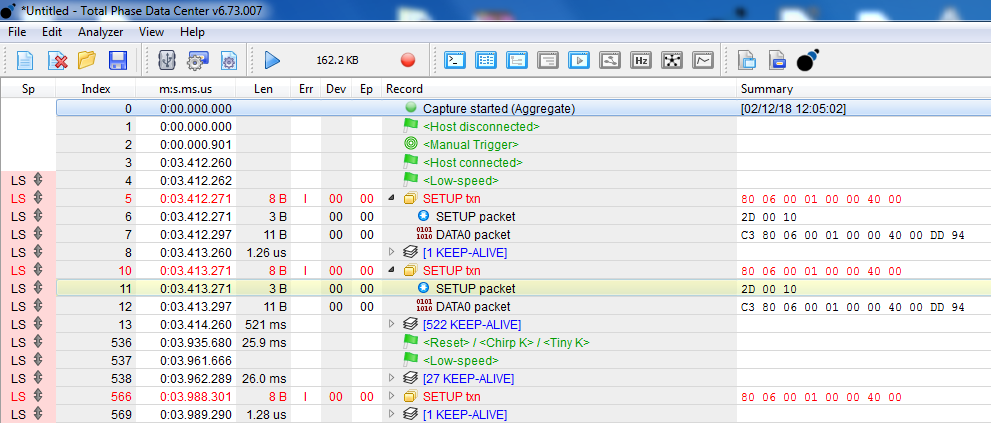
\includegraphics[width=12cm,height=6cm]{no_ACK_packets.PNG}
	\caption{Lack of ACK packets}
	\label{fig:Lack of ACK packets}
\end{figure}

\subsection{Trouble Shooting}

\begin{itemize}
	\item Make sure that the Nexys 3 Development Board's power switch is on, the switch can be found above 'A'
	\item Ensure that the USB port at 'A' is connected as this along with flashing the FPGA, supplies power to the Board.
	\item Is the Beagle 5000 switched on? You can tell by the TOTALPHASE LED found on device side, if it is not lit, the Beagle 5000 is not on. The switch is next to 'G'
	\item Over time, USB hubs become loose, have you ensured that there is a clear connection between devices? see figure \ref{fig:Loose Connection Evidence} as an example that could be evidence pointing to this problem.
	\item Nexys 3 Development Board not working? have you checked whether or not the constraints file has been included. If it has been included, there should be 4 LEDs on the board lit up after flashing.
\end{itemize}

\begin{figure}
	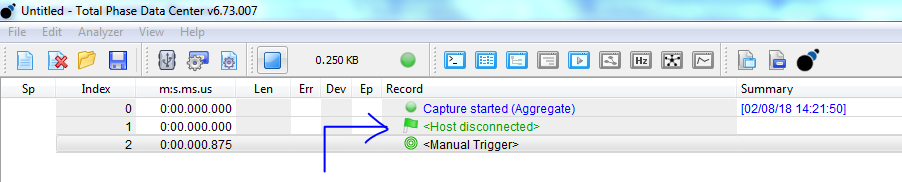
\includegraphics[width=12cm,height=4cm]{Loose_Connection_Evidence.PNG}
	\caption{Evidence of a loose connection}
	\label{fig:Loose Connection Evidence}
\end{figure}

\section{Reference Materials}
Here you can find documentation on the 
\href{https://reference.digilentinc.com/reference/programmable-logic/nexys-3/start}{Nexys 3 Development Board}
along with the .ucf file used to constrain the hardware design to certain pins. The webpage also includes a link to a 'Getting Started with FPGA" tutorial which may prove to be helpful. The Adept program used to flash the board can be found in this tutorial.\\

Git repositories for practice writing Verlog files can be found at \href{https://github.com/JammyJims/Verilog_Cores.git}{at this link here}, just clone the repository, import to Xilinx ISE and proceed to alter values/variables, and flash the FPGA.\\

USB core repository that I have set up made for this research can be found at my  \href{https://github.com/JammyJims/USB_Research.git}{other repository} This repository has my altered ROM file, Nexys 3 Top module, constraint file (.ucf extension). To download a fresh copy of the USB 1.1 function core that this researched is based on, follow \href{https://github.com/freecores/usb1_funct.git}{this link here}.\\

\href {https://stackoverflow.com/posts/48738506/edit}{Stackoverflow.com}, re-posted to \href {https://electronics.stackexchange.com/questions/355777/lack-of-ack-packets-appears-to-cause-custom-usb-core-to-not-work}{electronics.stackexchange.com} posts created regarding the lack of ACK packets issue found in the links above.\\

Materials on the USB 2.0 specification can be found at \href{http://www.usb.org/developers/docs/usb20_docs/}{www.usb.org}. Another good resource to reference would be the book: USB Complete The Developer's Guide by Jan Axelson, Dr Yuval Yarom has a copy of this book. Consider referencing \href {http://www.beyondlogic.org/usbnutshell/usb1.shtml}{USB in a NutShell} for the layout of device requests, and descriptors (Device/Configuration/Interface/Endpoint/String) 
\end{document}
